\section{\label{sec:group_primer}Group theory primer}

You may be already familiar with group theory.
If not so, the following textbooks are recommended as standard ones in the fields of physics and materials science.
\begin{itemize}
  \item \bibentry{dresselhaus2010group}
  \item \bibentry{el2008symmetry}
  \item \bibentry{Inui1996-et}
\end{itemize}
Here, we briefly prepare notations for group theory and introduce notions in crystallography in terms of group theory\footnote{
  We mainly adopt definitions in Refs.~\cite{ITA2016} and \cite{holt2005handbook}.
}.

\subsection{Definition}

% Group
\begin{screen}
  \begin{defn}[group \cite{holt2005handbook}]
    A \term{group} is a set $G$ with a binary operation $\circ: G \times G \to G$ that satisfies the following properties:
    \begin{itemize}
      \item (Closure) For all $g, h \in G$, $g \circ h \in G$;
      \item (Associativity) For all $g, h, k \in G$, $(g \circ h) \circ k = g \circ (h \circ k)$;
      \item (Identity) There exists a unique element $e \in G$ satisfying $g \circ e = e \circ g = g$ for all $g \in G$;
      \item (Inverse) For all $g \in G$, there exists an inverse of $g$, denoted by $g^{-1}$ such that $g \circ g^{-1} = g^{-1} \circ g = e$.
    \end{itemize}
  \end{defn}
\end{screen}

If a group $G$ is finite, the number of $G$ is called the \term{order} of $G$, denoted by $|G|$.
A subset of $G$ is called \term{generators} if all elements in $G$ can be written as a finite product of elements of the subset.
We write the products of group elements as $gh$ instead of $g \circ h$ as possible for conciseness.

% Example: affine group
We mention that the affine group $\mathcal{A}_{n}$ is group:
For $\begin{pmatrix} \bm{W}_{i} & \bm{w}_{i} \\ \bm{0}^{\top} & 1 \end{pmatrix} \in \mathcal{A}_{n} (i=1,2)$, the product of two affine mappings is also affine mapping,
\begin{align}
  \begin{pmatrix} \bm{W}_{1} & \bm{w}_{1} \\ \bm{0}^{\top} & 1 \end{pmatrix} \begin{pmatrix} \bm{W}_{2} & \bm{w}_{2} \\ \bm{0}^{\top} & 1 \end{pmatrix}
    &=
    \begin{pmatrix}
      \bm{W}_{1} \bm{W}_{2} & \bm{W}_{1} \bm{w}_{2} + \bm{w}_{1} \\
      \bm{0}^{\top} & 1
    \end{pmatrix}
    \in \mathcal{A}_{n}.
\end{align}
The associativity is followed by matrix multiplications.
The identity $ \begin{pmatrix} \bm{I}_{n} & \bm{0} \\ \bm{0}^{\top} & 1 \end{pmatrix}$ belongs to $\mathcal{A}_{n}$.
The inverse of an affine mapping is also an affine mapping,
\begin{align}
  \begin{pmatrix} \bm{W}_{1} & \bm{w}_{1} \\ \bm{0}^{\top} & 1 \end{pmatrix}
  &=
  \begin{pmatrix} \bm{W}_{1}^{-1} & -\bm{W}_{1}^{-1}\bm{w}_{1} \\ \bm{0}^{\top} & 1 \end{pmatrix} \in \mathcal{A}_{n}.
\end{align}

% Abelian group
\begin{screen}
  \begin{defn}[Abeliean group]
    A group $G$ is called \term{Abelian} if $g \circ h = h \circ g$ for all $g, h \in G$.
  \end{defn}
\end{screen}

% Example: translation group
A translation subgroup of $\mathcal{A}_{n}$ is an abelian group: for all $\bm{w}, \bm{w}' \in \mathbb{R}^{n}$,
\begin{align*}
  \begin{pmatrix} \bm{I}_{n} & \bm{w} \\ \bm{0}^{\top} & 1 \end{pmatrix}
  \begin{pmatrix} \bm{I}_{n} & \bm{w}' \\ \bm{0}^{\top} & 1 \end{pmatrix}
  =
  \begin{pmatrix} \bm{I}_{n} & \bm{w} + \bm{w}' \\ \bm{0}^{\top} & 1 \end{pmatrix}
  =
  \begin{pmatrix} \bm{I}_{n} & \bm{w}' \\ \bm{0}^{\top} & 1 \end{pmatrix}
  \begin{pmatrix} \bm{I}_{n} & \bm{w} \\ \bm{0}^{\top} & 1 \end{pmatrix}.
\end{align*}

\subsection{Subgroup}

% Subgroup
\begin{screen}
  \begin{defn}[subgroup \cite{holt2005handbook}]
    A subset $H$ of a group $G$ is called \term{subgroup} of $G$ if it forms a group under the same operation as that of $G$.
  \end{defn}
\end{screen}
We denote $H \leq G$ when a group $H$ is a subgroup of $G$.

The following criteria are commonly used to check a subset $H$ of group $G$ is a subgroup.
\begin{screen}
  \begin{prop}
    A subset $H$ of group $G$ is a subgroup of $G$ if and only if
    \begin{itemize}
      \item For all $h, h' \in H$, $hh' \in H$;
      \item and for all $h \in H$, $h^{-1} \in H$.
    \end{itemize}
  \end{prop}
\end{screen}
\begin{screen}
  \begin{prop}
    A subset $H$ of group $G$ is a subgroup of $G$ if and only if $h^{-1}h' \in H$ for all $h, h' \in H$.
  \end{prop}
\end{screen}

The Euclidean group is a subgroup of the affine group.
Let $\bm{G}$ be a metric tensor.
For $(\bm{W}, \bm{w}), (\bm{W}', \bm{w}') \in \mathcal{E}_{n}$, $\bm{W}^{\top} \bm{G} \bm{W} = \bm{G}$ and $\bm{W}'^{\top} \bm{G} \bm{W}' = \bm{G}$.
Then, $\bm{W}\bm{W}'$ gives an isometry affine mapping,
\begin{align*}
  (\bm{W}\bm{W}')^{\top} \bm{G} (\bm{W}\bm{W}')
    = \bm{W}'^{\top} (\bm{W}^{\top} \bm{G} \bm{W}) \bm{W}'
    = \bm{W}'^{\top} \bm{G} \bm{W}'
    = \bm{G}.
\end{align*}
For $(\bm{W}, \bm{w}) \in \mathcal{E}_{n}$, $\bm{G} = \bm{W}^{-\top} \bm{G} \bm{W}^{-1}$.
Thus, $\bm{W}^{-1}$ also gives an isometry affine mapping.

\subsection{Group action}

\subsubsection{Action}

\begin{screen}
  \begin{defn}[action]
    A \term{group action} of a group $G$ on a set $X$ is a mapping $\phi_{g}: X \to X$ for each $g \in G$ satisfying
    \begin{itemize}
      \item $\phi_{gh} = \phi_{g} \phi_{h}$ for all $g, h \in G$\footnote{
        This means $\phi_{gh}(x) = \phi_{g} (\phi_{h}(x))$ for all $x \in X$.
      };
      \item $\phi_{e}(x) = x$ for all $x \in X$.
    \end{itemize}
    Then, we say that $G$ \term{acts} on $X$.
  \end{defn}
\end{screen}
We write $\phi_{g}(x)$ as $gx$ in most cases.

The affine group $\mathcal{A}_{n}$ acts on the affine space $\mathbb{A}_{n}$.
Rather, we define the operation of affine mappings to be group action in Sec.~\ref{sec:affine_mapping_operation}.

\subsubsection{Orbit and crystallographic orbit}

\begin{screen}
  \begin{defn}[orbit]
    Let a group $G$ act on a set $X$.
    Two elements $x, y \in X$ lie in the same \term{orbit} under $G$ if there exists $g \in G$ such that $y = gx$.
    The set
    \begin{align}
      G(x) \coloneqq \set{gx}{g \in G}
    \end{align}
    is called the orbit of $x$ under $G$.
  \end{defn}
\end{screen}

\begin{screen}
  \begin{defn}[crystallographic orbit]
    An orbit under a space group is called a \term{crystallographic orbit}.
  \end{defn}
\end{screen}

The diagrams of plane groups in Fig.~\ref{fig:plane-group-diagrams} can be seen as orbits of points under each plane group.

\subsubsection{Stablilizer and site-symmetry group}

\begin{screen}
  \begin{defn}[stabilizer]
    Let a group $G$ act on $X$.
    The \term{stabilizer} of $x \in X$ in $G$ is
    \begin{align}
      \mathrm{Stab}_{G}(x) \coloneqq \set{ g \in G }{ gx = x }.
    \end{align}
  \end{defn}
\end{screen}
The stabilizer is a subgroup: for $g, h \in \mathrm{Stab}_{G}(x)$, $(g^{-1}h) x = g^{-1} (h x) = g^{-1}x = x$.

A space group acts on points in $\mathbb{R}^{n}$.
We consider classifying the points with respect to the action of the space group.
\begin{screen}
  \begin{defn}[site-symmetry group]
    The stabilizer of a point $\bm{x} \in \mathbb{R}^{n}$ on space group $\mathcal{G}$ is called \term{site-symmetry group} of $\bm{x}$.
  \end{defn}
\end{screen}

\begin{screen}
  \begin{defn}[General and special positions]
    A point $\bm{x} \in \mathbb{R}^{n}$ is called a point in a \term{general position} for a space group $\mathcal{G}$ if its site-symmetry group is identity.
    Otherwise, $\bm{x}$ is called a point in a \term{special position}.
  \end{defn}
\end{screen}

\paragraph{Example: site-symmetry groups on $pm$}

The symmetry operations of $pm$ are represented in augmented matrices as
\begin{align*}
  % t
  \left(
    \begin{array}{cc|c}
        1 & 0 & t_{1} \\
        0 & 1 & t_{2} \\
        \hline
        0 & 0 & 1 \\
    \end{array}
  \right),
  % m
  \left(
    \begin{array}{cc|c}
        -1 & 0 & t_{1} \\
        0  & 1 & t_{2} \\
        \hline
        0 & 0 & 1 \\
    \end{array}
  \right),
\end{align*}
where $t_{1}, t_{2} \in \mathbb{Z}$.
The fixed points of each symmetry operation are
\begin{itemize}
  \item $\left(
    \begin{array}{cc|c}
        1 & 0 & t_{1} \\
        0 & 1 & t_{2} \\
        \hline
        0 & 0 & 1 \\
    \end{array}
  \right)$: all points for $(t_{1}, t_{2}) = (0, 0)$, and nothing for otherwise;
  \item $\left(
    \begin{array}{cc|c}
        -1 & 0 & t_{1} \\
        0  & 1 & t_{2} \\
        \hline
        0 & 0 & 1 \\
    \end{array}
  \right)$: $(x, y) = (\frac{t_{1}}{2}, \ast)$ for $t_{2} = 0$, and nothing for otherwise.
\end{itemize}
Thus, site-symmetry groups of points in $\set{(x, y)}{ 0 \leq x < 1, 0 \leq y < 1}$ are
\begin{align*}
  \left(0, y\right):
    &\left\{
      \left( \begin{array}{cc|c}
        1 & 0 & 0 \\
        0 & 1 & 0 \\
        \hline
        0 & 0 & 1 \\
      \end{array} \right),
      \left( \begin{array}{cc|c}
        -1 & 0 & 0 \\
        0 & 1 & 0 \\
        \hline
        0 & 0 & 1 \\
      \end{array} \right)
    \right\} \\
  \left(\frac{1}{2}, y\right):
    &\left\{
      \left( \begin{array}{cc|c}
        1 & 0 & 0 \\
        0 & 1 & 0 \\
        \hline
        0 & 0 & 1 \\
      \end{array} \right),
      \left( \begin{array}{cc|c}
        -1 & 0 & 1 \\
        0 & 1 & 0 \\
        \hline
        0 & 0 & 1 \\
      \end{array} \right)
    \right\} \\
  \mbox{otherwise}:
      &\left\{
      \left( \begin{array}{cc|c}
        1 & 0 & 0 \\
        0 & 1 & 0 \\
        \hline
        0 & 0 & 1 \\
      \end{array} \right)
      \right\}.
\end{align*}
The points $(0, y)$ and $\left( \frac{1}{2}, y \right)$ are points in special positions.

\paragraph{Example: site-symmetry groups on $p2mg$}

The symmetry operations of $p2mg$ are represented in augmented matrices as
\begin{align*}
  % t
  \left(
    \begin{array}{cc|c}
        1 & 0 & t_{1} \\
        0 & 1 & t_{2} \\
        \hline
        0 & 0 & 1 \\
    \end{array}
  \right),
  % 2
  \left(
    \begin{array}{cc|c}
        -1 & 0 & t_{1} \\
        0  & -1 & t_{2} \\
        \hline
        0 & 0 & 1 \\
    \end{array}
  \right),
  % m
  \left(
    \begin{array}{cc|c}
        -1 & 0 & \frac{1}{2} + t_{1} \\
        0  & 1 & t_{2} \\
        \hline
        0 & 0 & 1 \\
    \end{array}
  \right),
  % a
  \left(
    \begin{array}{cc|c}
        1 & 0 & \frac{1}{2} + t_{1} \\
        0  & -1 & t_{2} \\
        \hline
        0 & 0 & 1 \\
    \end{array}
  \right),
\end{align*}
where $t_{1}, t_{2} \in \mathbb{Z}$.
The fixed points of each symmetry operation are
\begin{itemize}
  \item $\left(
    \begin{array}{cc|c}
        1 & 0 & t_{1} \\
        0 & 1 & t_{2} \\
        \hline
        0 & 0 & 1 \\
    \end{array}
  \right)$: all points for $(t_{1}, t_{2}) = (0, 0)$, and nothing for otherwise;
  \item $\left(
    \begin{array}{cc|c}
        -1 & 0 & t_{1} \\
        0  & -1 & t_{2} \\
        \hline
        0 & 0 & 1 \\
    \end{array}
  \right)$: $(x, y) = \left( \frac{t_{1}}{2}, \frac{t_{2}}{2} \right)$;
  \item $\left(
    \begin{array}{cc|c}
        -1 & 0 & \frac{1}{2} + t_{1} \\
        0  & 1 & t_{2} \\
        \hline
        0 & 0 & 1 \\
    \end{array}
  \right)$: $(x, y) = \left( \frac{t_{1}}{2} + \frac{1}{4}, \ast \right)$ for $t_{2} = 0$, and nothing for otherwise;
  \item $\left(
    \begin{array}{cc|c}
        1 & 0 & \frac{1}{2} + t_{1} \\
        0  & -1 & t_{2} \\
        \hline
        0 & 0 & 1 \\
    \end{array}
  \right)$: nothing.
\end{itemize}
Thus, site-symmetry groups of points in $\set{(x, y)}{ 0 \leq x < 1, 0 \leq y < 1}$ are
\begin{align*}
  (0, 0): &\left\{
    \left( \begin{array}{cc|c}
      1 & 0 & 0 \\
      0 & 1 & 0 \\
      \hline
      0 & 0 & 1 \\
    \end{array} \right),
    \left( \begin{array}{cc|c}
      -1 & 0 & 0 \\
      0 & -1 & 0 \\
      \hline
      0 & 0 & 1 \\
    \end{array} \right)
  \right\} \\
  \left( \frac{1}{2}, 0 \right): &\left\{
    \left( \begin{array}{cc|c}
      1 & 0 & 0 \\
      0 & 1 & 0 \\
      \hline
      0 & 0 & 1 \\
    \end{array} \right),
    \left( \begin{array}{cc|c}
      -1 & 0 & 1 \\
      0 & -1 & 0 \\
      \hline
      0 & 0 & 1 \\
    \end{array} \right)
  \right\} \\
  \left( 0, \frac{1}{2} \right): &\left\{
    \left( \begin{array}{cc|c}
      1 & 0 & 0 \\
      0 & 1 & 0 \\
      \hline
      0 & 0 & 1 \\
    \end{array} \right),
    \left( \begin{array}{cc|c}
      -1 & 0 & 0 \\
      0 & -1 & 1 \\
      \hline
      0 & 0 & 1 \\
    \end{array} \right)
  \right\} \\
  \left( \frac{1}{2}, \frac{1}{2} \right): &\left\{
    \left( \begin{array}{cc|c}
      1 & 0 & 0 \\
      0 & 1 & 0 \\
      \hline
      0 & 0 & 1 \\
    \end{array} \right),
    \left( \begin{array}{cc|c}
      -1 & 0 & 1 \\
      0 & -1 & 1 \\
      \hline
      0 & 0 & 1 \\
    \end{array} \right)
  \right\} \\
  \left( \frac{1}{4}, y \right): &\left\{
    \left( \begin{array}{cc|c}
      1 & 0 & 0 \\
      0 & 1 & 0 \\
      \hline
      0 & 0 & 1 \\
    \end{array} \right),
    \left( \begin{array}{cc|c}
      -1 & 0 & 0 \\
      0 & 1 & 0 \\
      \hline
      0 & 0 & 1 \\
    \end{array} \right)
  \right\} \\
  \left( \frac{3}{4}, y \right): &\left\{
    \left( \begin{array}{cc|c}
      1 & 0 & 0 \\
      0 & 1 & 0 \\
      \hline
      0 & 0 & 1 \\
    \end{array} \right),
    \left( \begin{array}{cc|c}
      -1 & 0 & 1 \\
      0 & 1 & 0 \\
      \hline
      0 & 0 & 1 \\
    \end{array} \right)
  \right\} \\
  \mbox{otherwise}: &\left\{
    \left( \begin{array}{cc|c}
      1 & 0 & 0 \\
      0 & 1 & 0 \\
      \hline
      0 & 0 & 1 \\
    \end{array} \right)
  \right\}.
\end{align*}
The points $(0, 0)$, $\left( \frac{1}{2}, 0 \right)$, $\left( 0, \frac{1}{2} \right)$, $\left( \frac{1}{2}, \frac{1}{2} \right)$, $\left( \frac{1}{4}, y \right)$, and $\left( \frac{3}{4}, y \right)$ are points in special positions.

\subsection{Isomorphism and conjugacy}

\subsubsection{Isomoprhism}

\begin{screen}
  \begin{defn}[isomorphism]
    Let $G$ and $H$ be groups.
    A bijection $\phi: G \to H$ is called \term{isomorphism} if $\phi(gg') = \phi(g) \phi(g')$ for all $g, g' \in G$.
    If an isomorphism exists between $G$ and $H$, they are called \term{isomorphic} and denoted by $G \cong H$.
  \end{defn}
\end{screen}

The translation subgroup of $\mathcal{A}_{n}$ is isomorphic to $\mathbb{R}^{n}$ by the bijection $\mathcal{T}_{n} \ni (\bm{I}_{n}, \bm{w}) \mapsto \bm{w} \in \mathbb{R}^{n}$.

\subsubsection{\label{sec:conjugation_wyckoff}Conjugacy subgroup and Wyckoff position}

Let us classify subgroups of group $G$.
First, we consider an action of $G$ on $G$.
\begin{screen}
  \begin{defn}[conjugation]
    Let $G$ be a group.
    The action of $G$ on $G$,
    \begin{align}
      \bullet^{g}: G \ni h \mapsto h^{g} \coloneqq g^{-1} h g \in G,
    \end{align}
    is called \term{conjugation}\footnote{
      Check $h^{gg'} = (h^{g})^{g'}$.
    }.
    The orbits of the actions are called \term{conjugacy classes} of $G$.
    Elements in the same conjugacy class are called to be \term{conjugate} in $G$.
  \end{defn}
\end{screen}

The conjugation gives an equivalence relationship between subgroups.
\begin{screen}
  \begin{defn}[conjugate subgroup]
    Let $H$ be a subgroup of $G$.
    The set
    \begin{align}
      H^{g} \coloneqq g^{-1} H g = \set{ h^{g} }{ h \in H}
    \end{align}
    is an isomorphic subgroup to $H$, which called a \term{conjugate subgroup}.
  \end{defn}
\end{screen}

Now, consider classifying points in special positions more finely.
We observe each point in a crystallographic orbit under a space group $\mathcal{G}$ gives a conjugate subgroup to each other: for $\bm{x} = g \bm{y}$,
\begin{align}
  \mathrm{Stab}_{\mathcal{G}}(\bm{y})
    &= \set{ h \in G }{ ghg^{-1}\bm{x} = \bm{x} } \nonumber \\
    &= \set{ g^{-1} h g }{ h \in \mathrm{Stab}_{\mathcal{G}}(\bm{x}) } \nonumber \\
    &= g^{-1} \circ \mathrm{Stab}_{\mathcal{G}}(\bm{x}) \circ g.
\end{align}

The conjugate subgroups motivate the classification of site-symmetry groups by conjugations.
\begin{screen}
  \begin{defn}[Wyckoff position]
    Two points $\bm{x}$ and $\bm{y}$ belong to the same \term{Wyckoff position} for a space group $\mathcal{G}$ if their site-symmetry groups are conjugate subgroups of $\mathcal{G}$.
  \end{defn}
\end{screen}

Note that the Wyckoff position of $\bm{x}$ contains all the points in $\mathcal{G}(\bm{x})$.
Also, two points in different orbits will belong to the same Wyckoff position.
For example, all points in general positions belong to the same Wyckoff position.

\begin{figure}[htb]
  \centering
  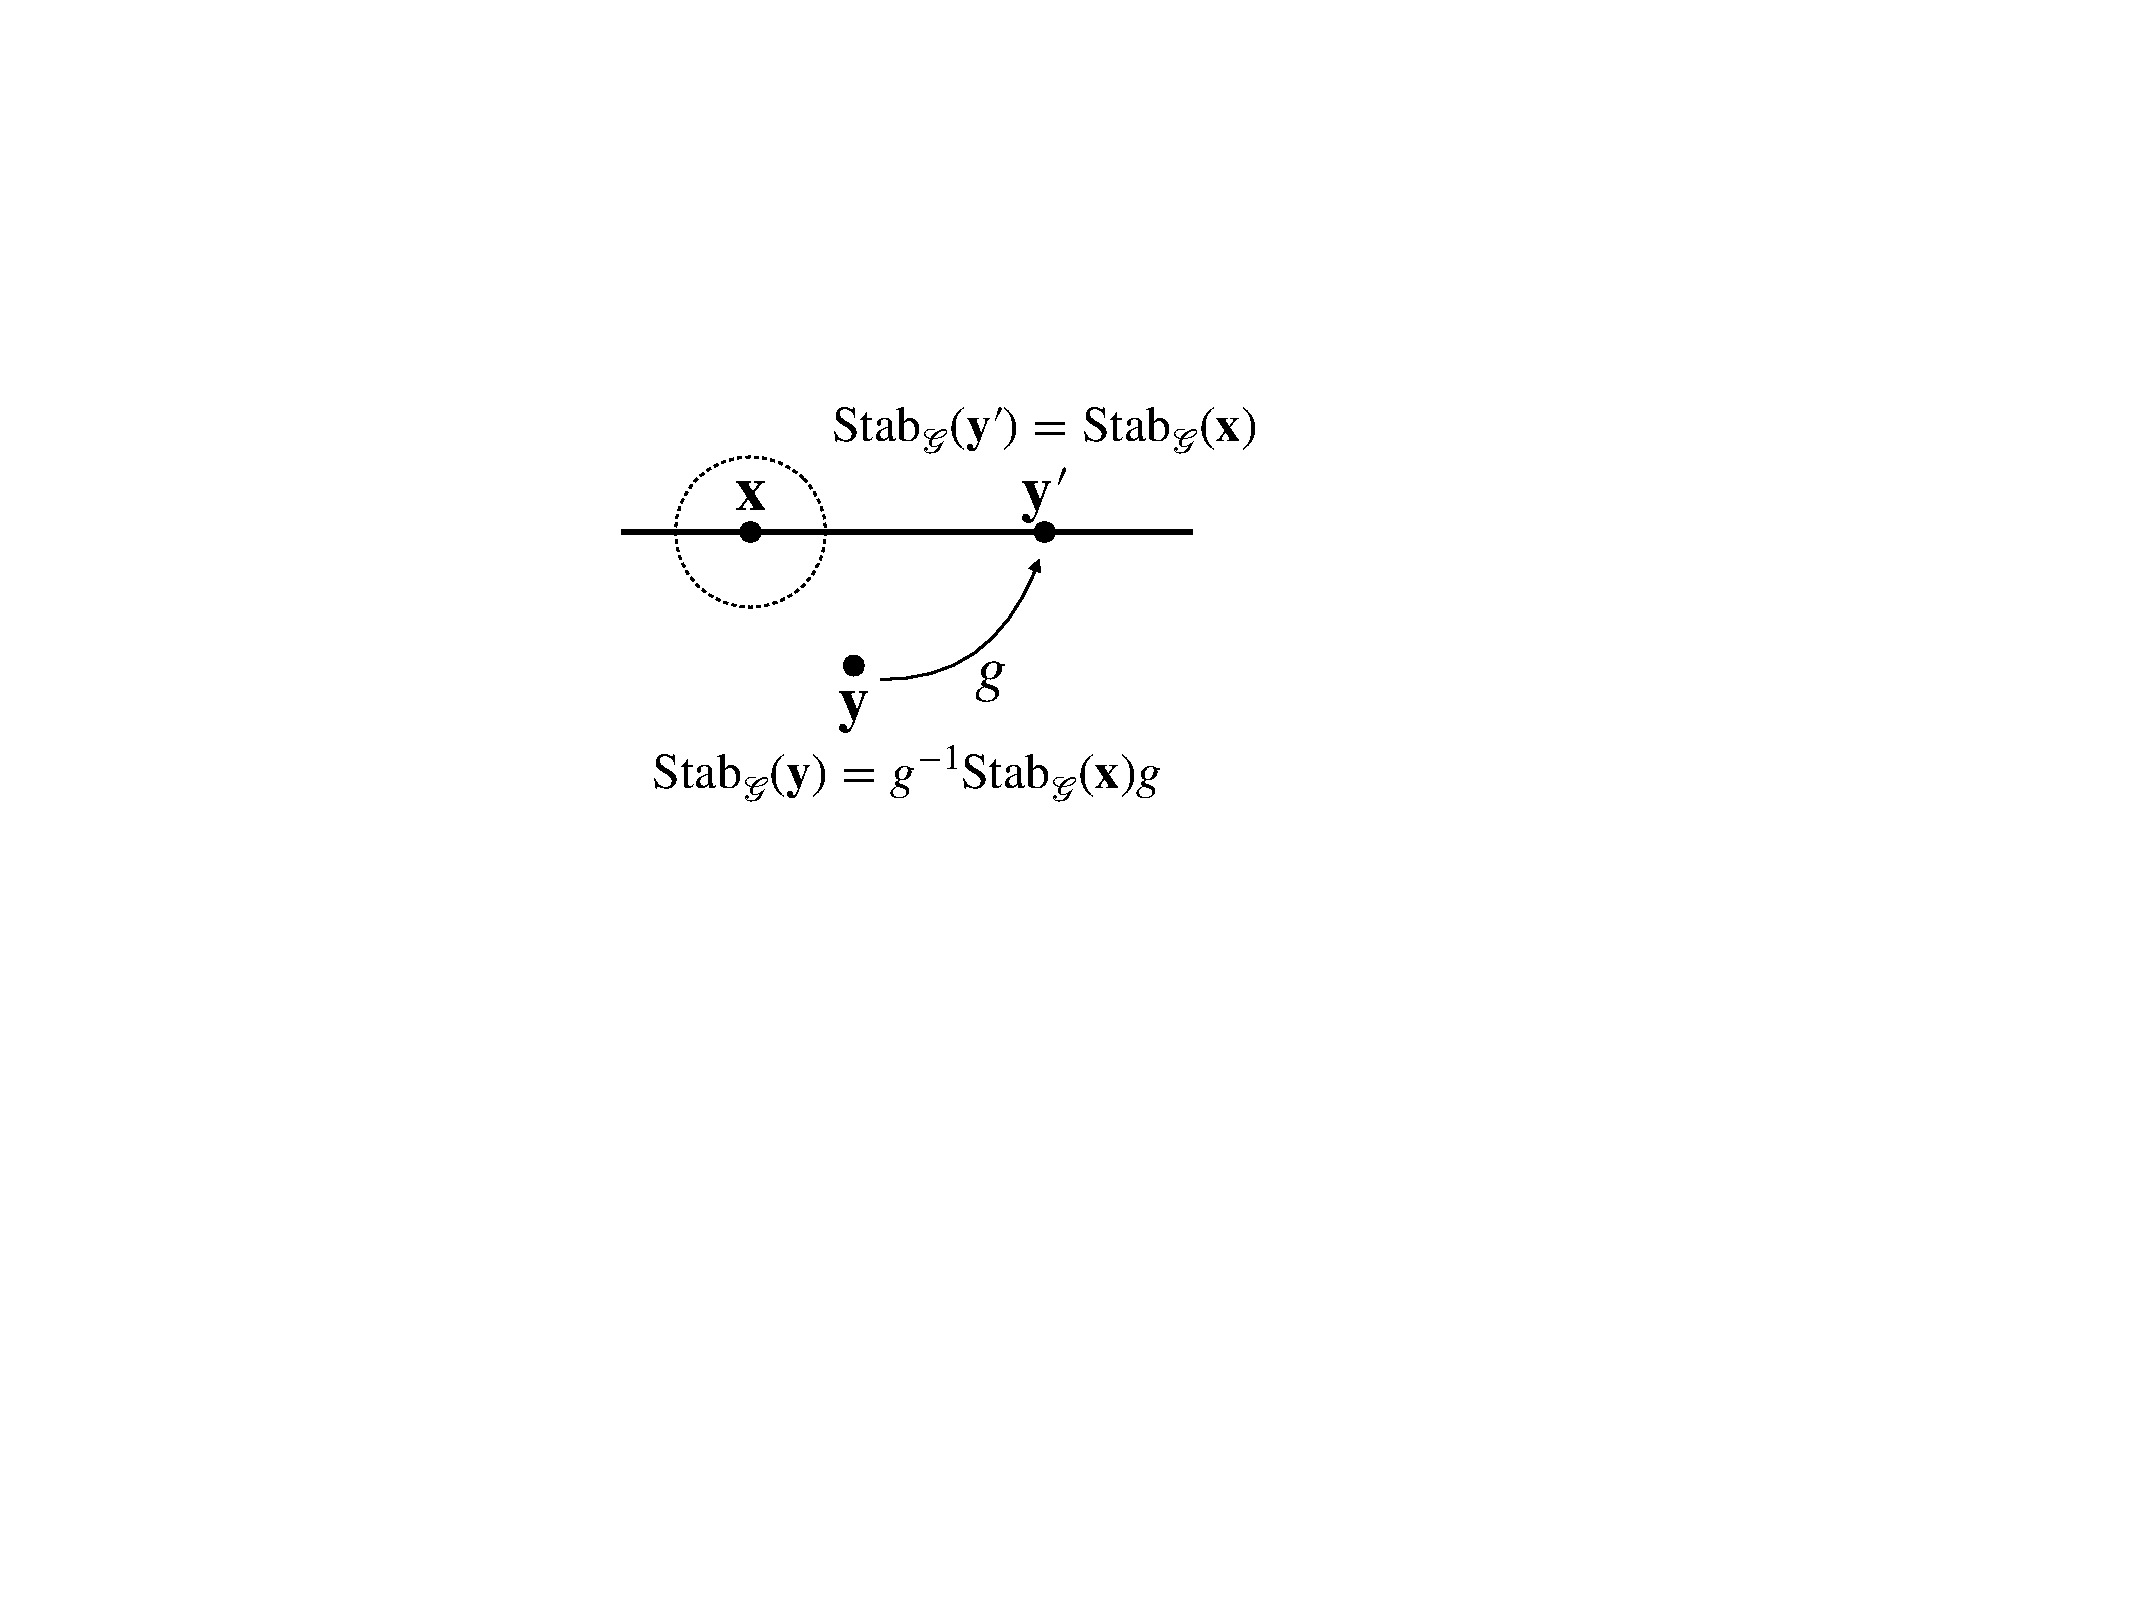
\includegraphics[width=0.4\textwidth]{figure/fig_wyckoff.pdf}
  \caption{The Wyckoff position for an isolated point is identical to its crystallographic orbit.}
  \label{fig:isolated-wyckoff-position}
\end{figure}

If a point $\bm{x}$ has a different site-symmetry group than its neighbor, the points belonging to the Wyckoff position are identical to the orbit of $\bm{x}$.
We can prove this by contradiction (see Fig.~\ref{fig:isolated-wyckoff-position} for sketch of proof).
Let $\bm{x}$ be a point with a different site-symmetry group than its neighbor.
Suppose a point $\bm{y}$ has a conjugate subgroup $\mathrm{Stab}_{\mathcal{G}}(\bm{y}) = g^{-1}  \mathrm{Stab}_{\mathcal{G}}(\bm{x}) g$, but $\bm{x}$ and $\bm{y}$ do not belong to the same crystallographic orbit.
Then, the site-symmetry group of $\bm{y}' = g\bm{x}$ is $\mathrm{Stab}_{\mathcal{G}}(\bm{y}') = g \mathrm{Stab}_{\mathcal{G}}(\bm{x}) g^{-1} = \mathrm{Stab}_{\mathcal{G}}(\bm{x})$.
Then, $\bm{x}$ and $\bm{y}'$ are different points by assumption.
Because the points in a line connecting $\bm{x}$ and $\bm{y}'$ have the same site-symmetry group with $\mathrm{Stab}_{\mathcal{G}}(\bm{x})$, there is a neighbor point of $\bm{x}$ that has the same site-symmetry group with $\bm{x}$, which is a contradiction.

The Wyckoff positions are often displayed with \term{Wyckoff multiplicity} and \term{Wyckoff letter}.
The Wyckoff multiplicity denotes the number of points in a crystallographic orbit lying in the conventional cell.
The Wyckoff letter labels each Wyckoff position by a single letter starting from ``a''\footnote{
  \href{https://www.cryst.ehu.es/cgi-bin/cryst/programs/nph-wp-list}{$Pmmm$ (No. 47)} has 27 Wyckoff positions.
  Thus, the Latin alphabet is not enough for Wyckoff letters.
}.

\paragraph{Example: Wyckoff positions of $pm$}

\begin{itemize}
  \item $(0, y)$ $\Rightarrow$ $1a$
  \item $\left( \frac{1}{2}, y \right)$ $\Rightarrow$ $1b$
  \item otherwise $\Rightarrow$ $2c$
\end{itemize}

\paragraph{Example: Wyckoff positions of $p2mg$}

\begin{itemize}
  \item $(0, 0)$, $\left( \frac{1}{2}, 0 \right)$ $\Rightarrow$ $2a$
  \item $\left( 0, \frac{1}{2} \right)$, $\left( \frac{1}{2}, \frac{1}{2} \right)$ $\Rightarrow$ $2b$
  \item $\left( \frac{1}{4}, y \right)$, $\left( \frac{3}{4}, y \right)$ $\Rightarrow$ $2c$
  \item otherwise $\Rightarrow$ $4d$
\end{itemize}

\subsection{Coset, normal subgroup, and factor group}

\begin{screen}
  \begin{defn}[coset]
    Let $H$ be a subgroup of $G$.
    For $g \in G$, the subset
    \begin{align}
      gH \coloneqq \set{ gh }{ h \in H}
    \end{align}
    is called the \term{left coset} of $H$ with \term{representative} $g$.
  \end{defn}
\end{screen}
The coset $eH$ is $H$ itself.
Two cosets $gH$ and $g'H$ are equal if and only if $g^{-1}g' \in H$.
Otherwise, $gH$ and $g'H$ are disjoint.

A group can be decomposed into disjointed cosets,
\begin{align}
  G = \bigsqcup_{i} g_{i} H.
\end{align}

\begin{screen}
  \begin{defn}[normal subgroup]
    A subgroup $N$ of group $G$ is called \term{normal} if $N^{g} = N$ for all $g \in G$, denoted as $N \trianglelefteq G$.
  \end{defn}
\end{screen}

The normal subgroup is characterized by the property that the product of any $gn \in gN$ and $g'n' \in g'N$ belongs to $gg'N$\footnote{
  If $N$ is normal, $(gn)(g'n') = (gg')(g'^{-1} n g') n' \in gg' N$.
}.

\begin{screen}
  \begin{defn}[factor group]
    The \term{factor group} of group $G$ by normal subgroup $N$ is a set of cosets $gN \, (g \in G)$ with the binary operation, $gH \circ g'H = gg' H$.
  \end{defn}
\end{screen}

The translation subgroup $\mathcal{T}_{n}$ is a normal subgroup of $\mathcal{A}_{n}$,
\begin{align*}
  \begin{pmatrix} \bm{W} & \bm{w} \\ \bm{0}^{\top} & 1 \end{pmatrix}^{-1}
  \begin{pmatrix} \bm{I}_{n} & \bm{t} \\ \bm{0}^{\top} & 1 \end{pmatrix}
  \begin{pmatrix} \bm{W} & \bm{w} \\ \bm{0}^{\top} & 1 \end{pmatrix}
  =
  \begin{pmatrix} \bm{I}_{n} & \bm{W}^{-1} \bm{t} \\ \bm{0}^{\top} & 1 \end{pmatrix}
  \in \mathcal{T}_{n}.
\end{align*}

\subsection{homomorphism, kernel, image}

\begin{screen}
  \begin{definition}[homomorphism]
    Let $G$ and $H$ be groups.
    A map $\phi: G \to H$ is called \term{homomorphism} if $\phi(gg') = \phi(g) \phi(g')$ for all $g, g' \in G$.
  \end{definition}
\end{screen}

\begin{screen}
  \begin{definition}[kernel]
    Let $\phi: G \to H$ be a homomorphism between groups $G$ and $H$.
    The set
    \begin{align}
      \mathrm{Ker}(\phi) \coloneqq \set{ g \in G }{ \phi(g) = e }
    \end{align}
    is called a \term{kernel} of $\phi$.
  \end{definition}
\end{screen}

\begin{screen}
  \begin{prop}
    Let $\phi: G \to H$ be a homomorphism between groups $G$ and $H$.
    The kernel $\mathrm{Ker}(\phi)$ is a normal subgroup of $G$.
  \end{prop}
\end{screen}

\begin{screen}
  \begin{definition}[image]
    Let $\phi: G \to H$ be a homomorphism between groups $G$ and $H$.
    The set
    \begin{align}
      \mathrm{Im}(\phi) \coloneqq \set{ \phi(g) }{ g \in G }
    \end{align}
    is called an \term{image} of $\phi$.
  \end{definition}
\end{screen}

\begin{screen}
  \begin{prop}
    Let $\phi: G \to H$ be a homomorphism between groups $G$ and $H$.
    The image $\mathrm{Im}(\phi)$ is a subgroup of $H$.
  \end{prop}
\end{screen}

\begin{screen}
  \begin{them}[first isomorphism theorem]
    Let $\phi: G \to H$ be a homomorphism between groups $G$ and $H$.
    Let $N$ be the kernel of $\phi$.
    There is an isomorphism $G/N \ni gN \mapsto \phi(g) \in \mathrm{Im}(\phi)$.
    That is, $G/N \cong \mathrm{Im}(\phi)$.
  \end{them}
\end{screen}

We can construct a homomorphism between $\mathcal{E}_{n}$ and $\mathrm{O}(n)$ as
\begin{align*}
  \varphi: \mathcal{E}_{n} \ni \begin{pmatrix} \bm{W} & \bm{w} \\ \bm{0}^{\top} & 1 \end{pmatrix}
    \mapsto \bm{A} \bm{W} \bm{A}^{-1} \in \mathrm{O}(n).
\end{align*}
The kernel of $\varphi$ is
\begin{align*}
  \mathrm{Ker}(\varphi) = \mathcal{T}_{n}.
\end{align*}
Thus, $\mathcal{A}_{n} / \mathcal{T}_{n}$ is isomorphic to $\mathrm{O}(n)$.
